
\section{Optimal thresholds}
For a given coalition $\C$, there are countless possible choices for an institutional design $f$ that computes the aggregated decision based on coalition members' votes. As mentioned earlier, this function $f$ allways introduces a tradeoff between credible deterrence and excalation controll. 

For $\C$ then, it is highly important to understand which such designs that give the best deterrence credibility while minimizing the risk of accidental retaliation. In essence, this is the classical tradeoff between the probability of \emph{true positives} and the probability of \emph{false positives}. There is a rich history from many fields of science studying this exact tradeoff, see for example \citeme and \citeme, that we can use to study this issue in our setting.

Our choice function $f$ has two possible outcomes, retaliation or no retaliation, based on two possible situations of true or false attacks. By false attack, or no attack, we here mean that there has been a false detection due to an accident, or an attack that is misattributed to the wrong adversary. This means that the function $f$ is a binary classifier, in the sense of \citeme. 

The standard way of measuring the accuracy of a binary classifier is to measure the correct and incorrect assignments. For this we have a simple contingency matrix:

\begin{table}[h]
\centering
\begin{tabular}{l|ll}
    & Retaliation & No retaliation \\ \hline
    Attack & True positive & False negative       \\
    No attack & False positive & True negative
\end{tabular}
\end{table}

This gives us the \emph{true positive rate} (TPR), defined as 
\[\mathrm{TPR} = \frac{\text{true positive}}{\text{true positive} + \text{false negative}}\]
and the \emph{false positive rate} (FPR), defined as 
\[\mathrm{FPR} = \frac{\text{false negative}}{\text{true positive} + \text{false negative}}.\]
These are, respectively, the probability that retaliation occurs, and the probability of an accidental retaliation, which we have previously named $R(\tau)$ and $F(\tau)$. 

The binary classifier is dependent on the threshold $\tau$, which allows us to visualize the classifiers performance on the true positive-false positive tradeoff by ROC curves. 

\subsection{ROC curves}
Reciever Operating Characteristic (ROC) curves were first used for radar signals during World War II, where they were used as an analysis tool for strengthening the predicting power of radars after the Pearl Harbor attack \citeme. Since then they have dound a wide use throughout science, mainly in medicine \citeme, epidemiology \citeme, and more recently as a tool for evaluating classification algorithms in machine learning \citeme and artificial intelligence \citeme. 

The ROC space is defined by having TPR and FPR as its axes, and as these are rates from $0$ to $1$ the space is equivalent to the unit square. Any point in this space represents a tradeoff between true positives and false positives. The point $(0,1)$ is the \emph{perfect classifier}, in the sense that it correctly identifies $100\%$, with $0\%$ errors. The diagonal line $(x,x)$ represents a random classifier. Hence, points above the diagonal are better than random guessing, and points below are worse. 

By plotting $(F(\tau), R(\tau))$ for all different thresholds $\tau$, one gets a curve through ROC space that visualizes the effect of the threshold on the true positive-false positive tradeoff. The point on this curve that is closest to the perfect classifier $(0,1)$ is the optimal threshold for the given choice function. 

By making ROC curves for a variety of choice functions, we can then identify the \emph{best} institutional design for the coalition $\C$, in terms of maximizing correct retaliations while minimizing accidental use. One method for doing this is comparing ROC rurves on their area under the curve (AUC) -- a better institutional design will have a larger AUC. 

We do this in two different situations: a large coalition and a small coalition. For the small coalition the small number of members allow us to compute the ROC curves empirically for a variety of choice functions $f$. For large coalitions, however, we use a normal approximation to the probabilities, and plot binormal ROC curves, as in \citeme, instead. 


\subsection{Small coalitions}
Our small coalition $\C$ will consit of four members. We will not go into specifics or create a realistic coalition here, as this paper only serves to demonstrate the effect of the institutional design on the deterrence mechanism, and not imply policy. This also allow us to test hypothetical alterations of the choice functions due to different contexts the coalition exists in; specifically we consider choice function weight vectors $w$ based on hypothetical geographical, technological and geopolitical contexts. 

The ROC curves are dependent on the probabilities of correct indentification and the coalition members belief about the type $T$ of the adversary state $\A$. In order to compare choice functions based on their performance, we plot choice functions based on several natural weight schemes $w = [w_1, w_2, w_3, w_4]$ at the same time -- for fixed probability vectors $p = [p_1, p_2, p_3, p_4]$ and $q = [q_1, q_2, q_3, q_4]$. 

We have chosen five different weight schemes for our coalition $\C = \{1,2,3,4\}$, which we will use for all of the probability variations. We have normalized them so that they all have the same total sum of $4$, as well as put the weights in decreasing order for simplicity. 
\begin{enumerate}
    \item $w = (1,1,1,1)$ -- the \emph{unbiased} scheme. This treats all coalition members equally. Varying the threshold $\tau$ then gives the standard voting schemes described in \cref{ssec:threshold-rules}. 
    \item $w = (4,0,0,0)$ -- the \emph{dictator} scheme. This is essentially the shared capability structure employed by NATO today, where the country owning the deterrence technology also has full control over its use.  
    \item $w = (2.5, 0.5, 0.5, 0.5)$ -- the \emph{veto} scheme. The scheme allows a single member to have full veto rights for most thresholds. 
    \item $w = (1.16, 1.06, 0.89, 0.89)$ -- the \emph{technology} scheme. This weighs members according to bias coming from assymetric qualities, like techonology, competencies, or ISR capabilities. 
    \item $w = (1.6, 0.8, 0.8, 0.8)$ -- the \emph{frontline} scheme. This scheme weighs, for example, a coalition member that is a border-state with the adversary higher than the other members. 
    \item $w = (1.6, 1.2, 0.8, 9.4)$ -- the \emph{geographical} scheme. The scheme weighs members according to their distance from the agressor, and hence by the probability of being affected. 
    \item $w = (1.33, 1.33, 0.67, 0.67)$ -- the \emph{two-bloc} scheme. This represents a coalition where there are two main members forming a block, and two secondary members forming a second block. 
\end{enumerate}

To have a base line, we look at the case where all coalition members have the same probability of voting in favor of retaliation given the type of $\A$. The following shows the ROC curves for the above weight schemes when both the shared resolve and the accuracy for correct identification are \emph{high} -- represented by $p = [0.85, 0.85, 0.85, 0.85]$ and $q = [0.05, 0.05, 0.05, 0.05]$ -- and when the shared resolve and accuracy is \emph{low} -- represented by $p = [0.60, 0.60, 0.60, 0.60]$ and $q = [0.20, 0.20, 0.20, 0.20]$. 

\begin{figure}[h!]
    \centering
    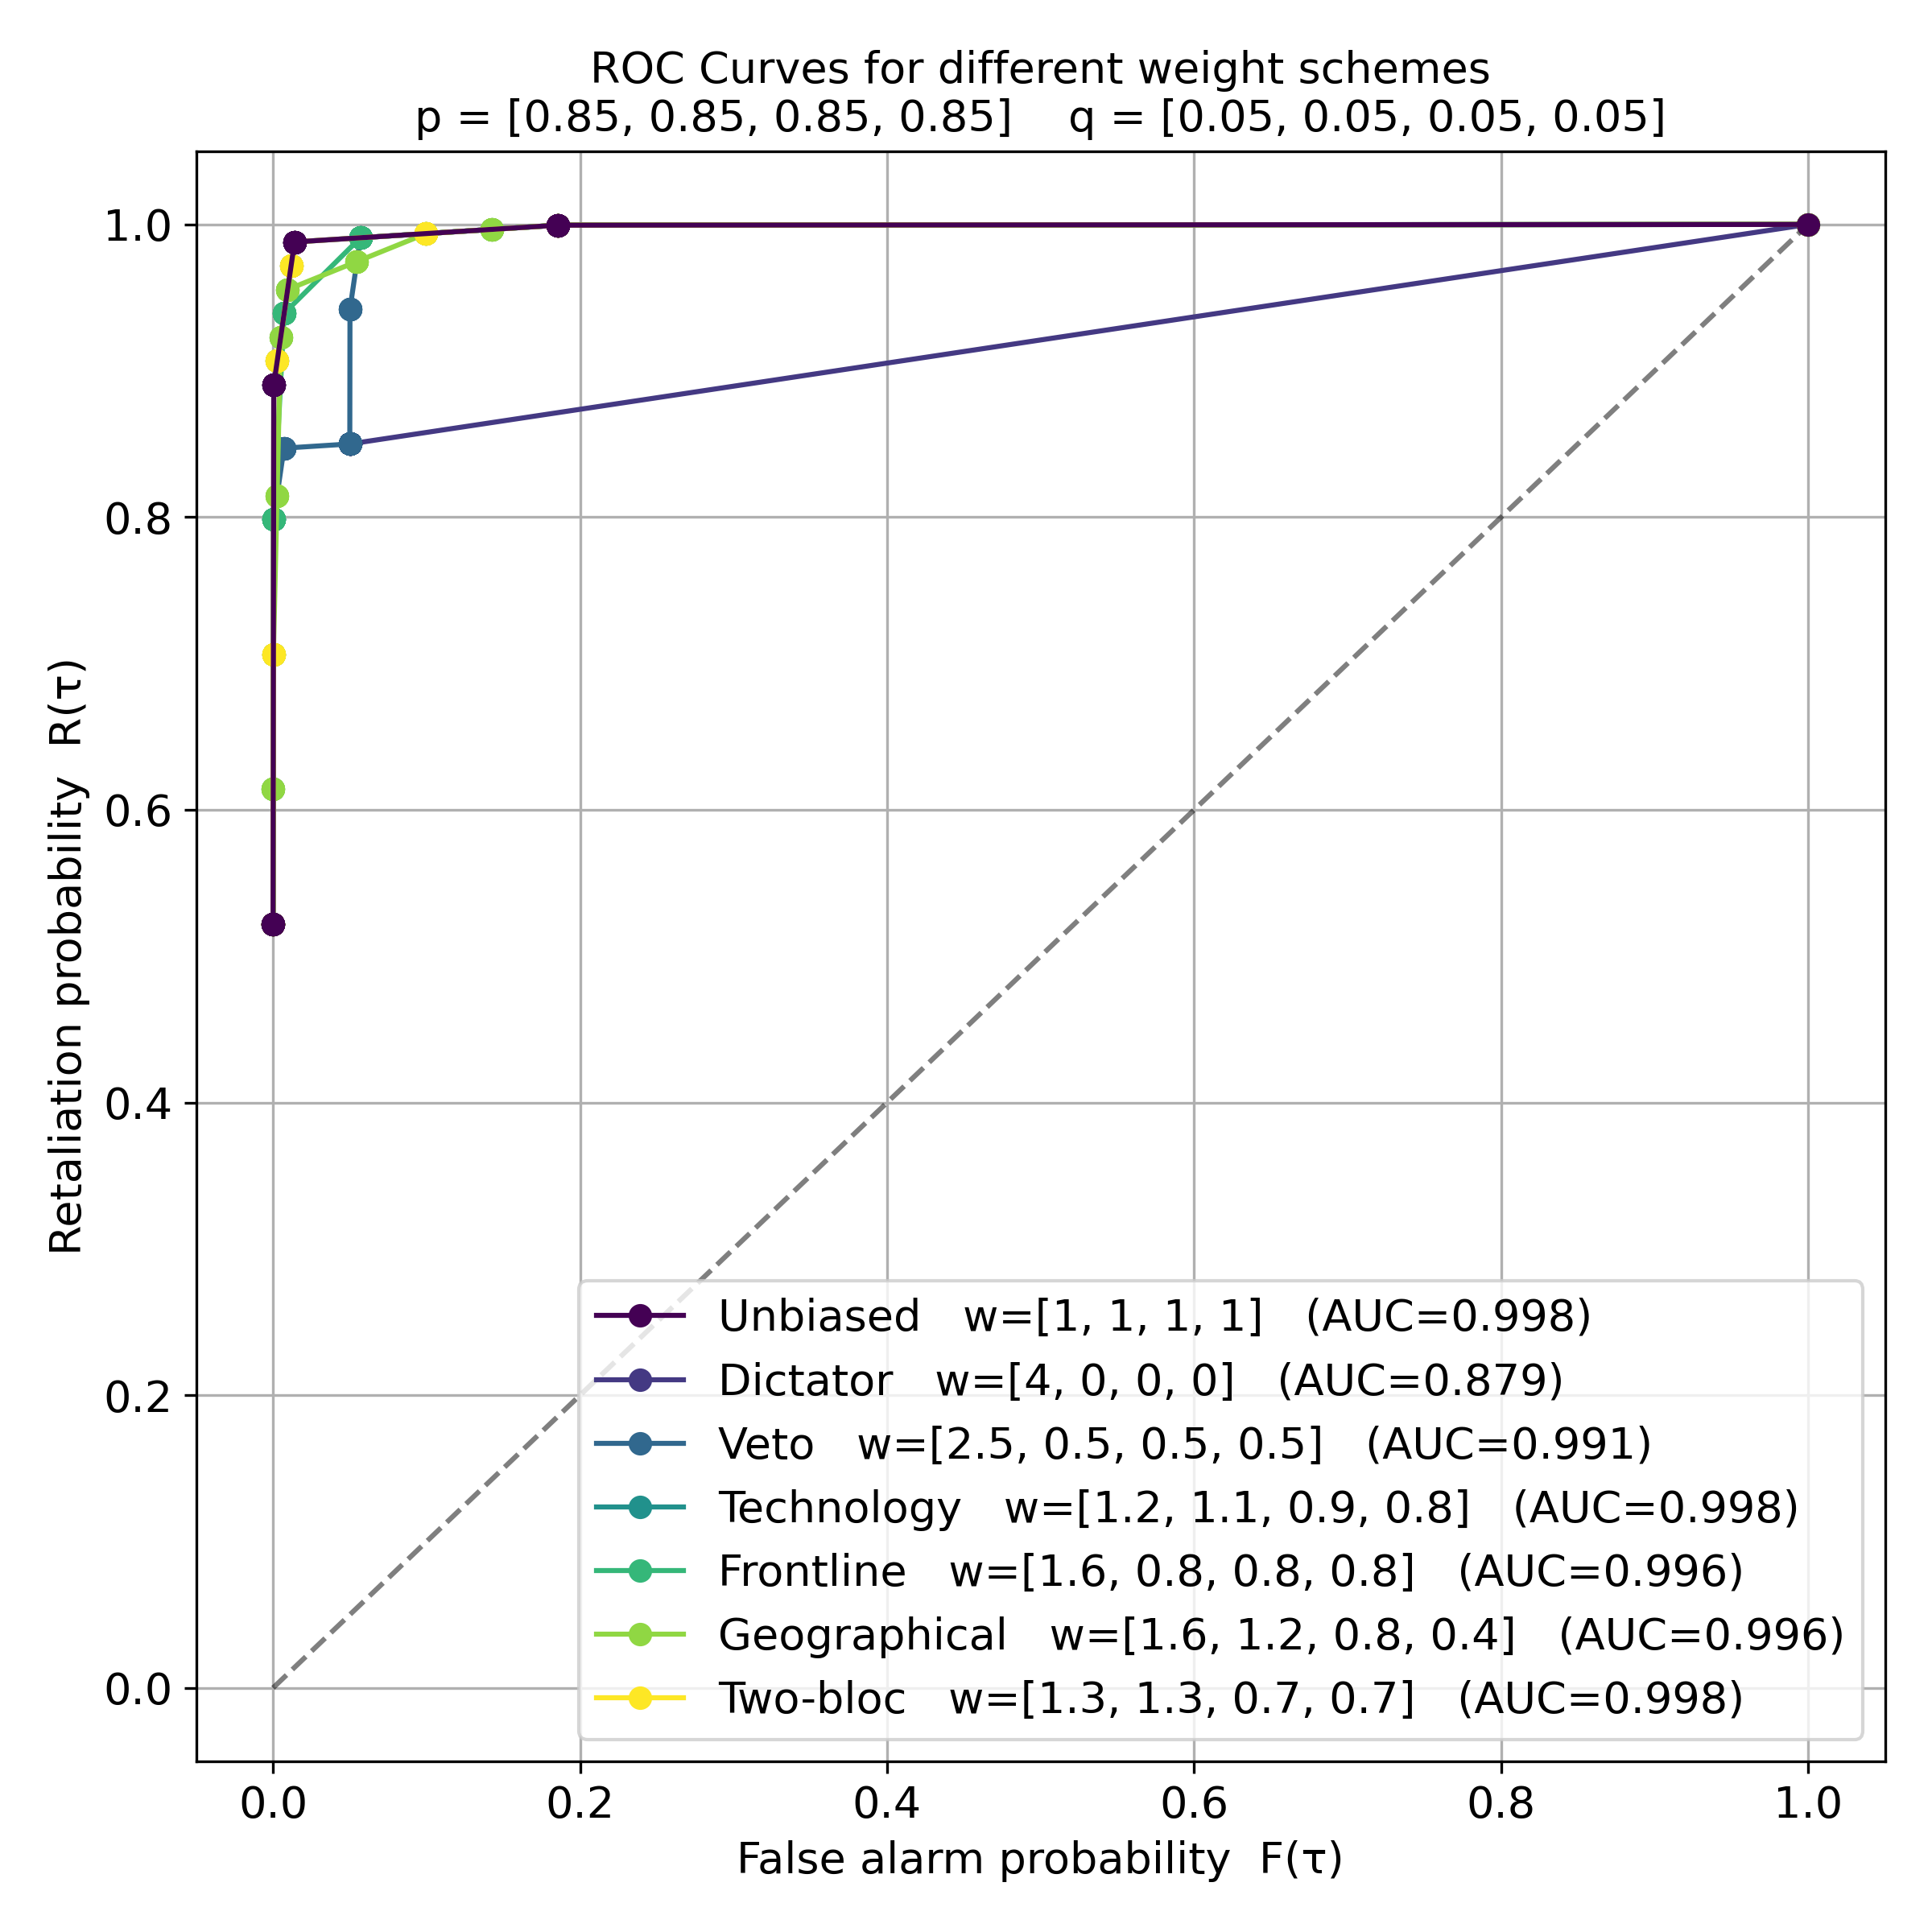
\includegraphics[width=\columnwidth]{images/ROC_HighSymmetric.png.png}
    \label{fig:high-high}
\end{figure}

\begin{figure}[h!]
    \centering
    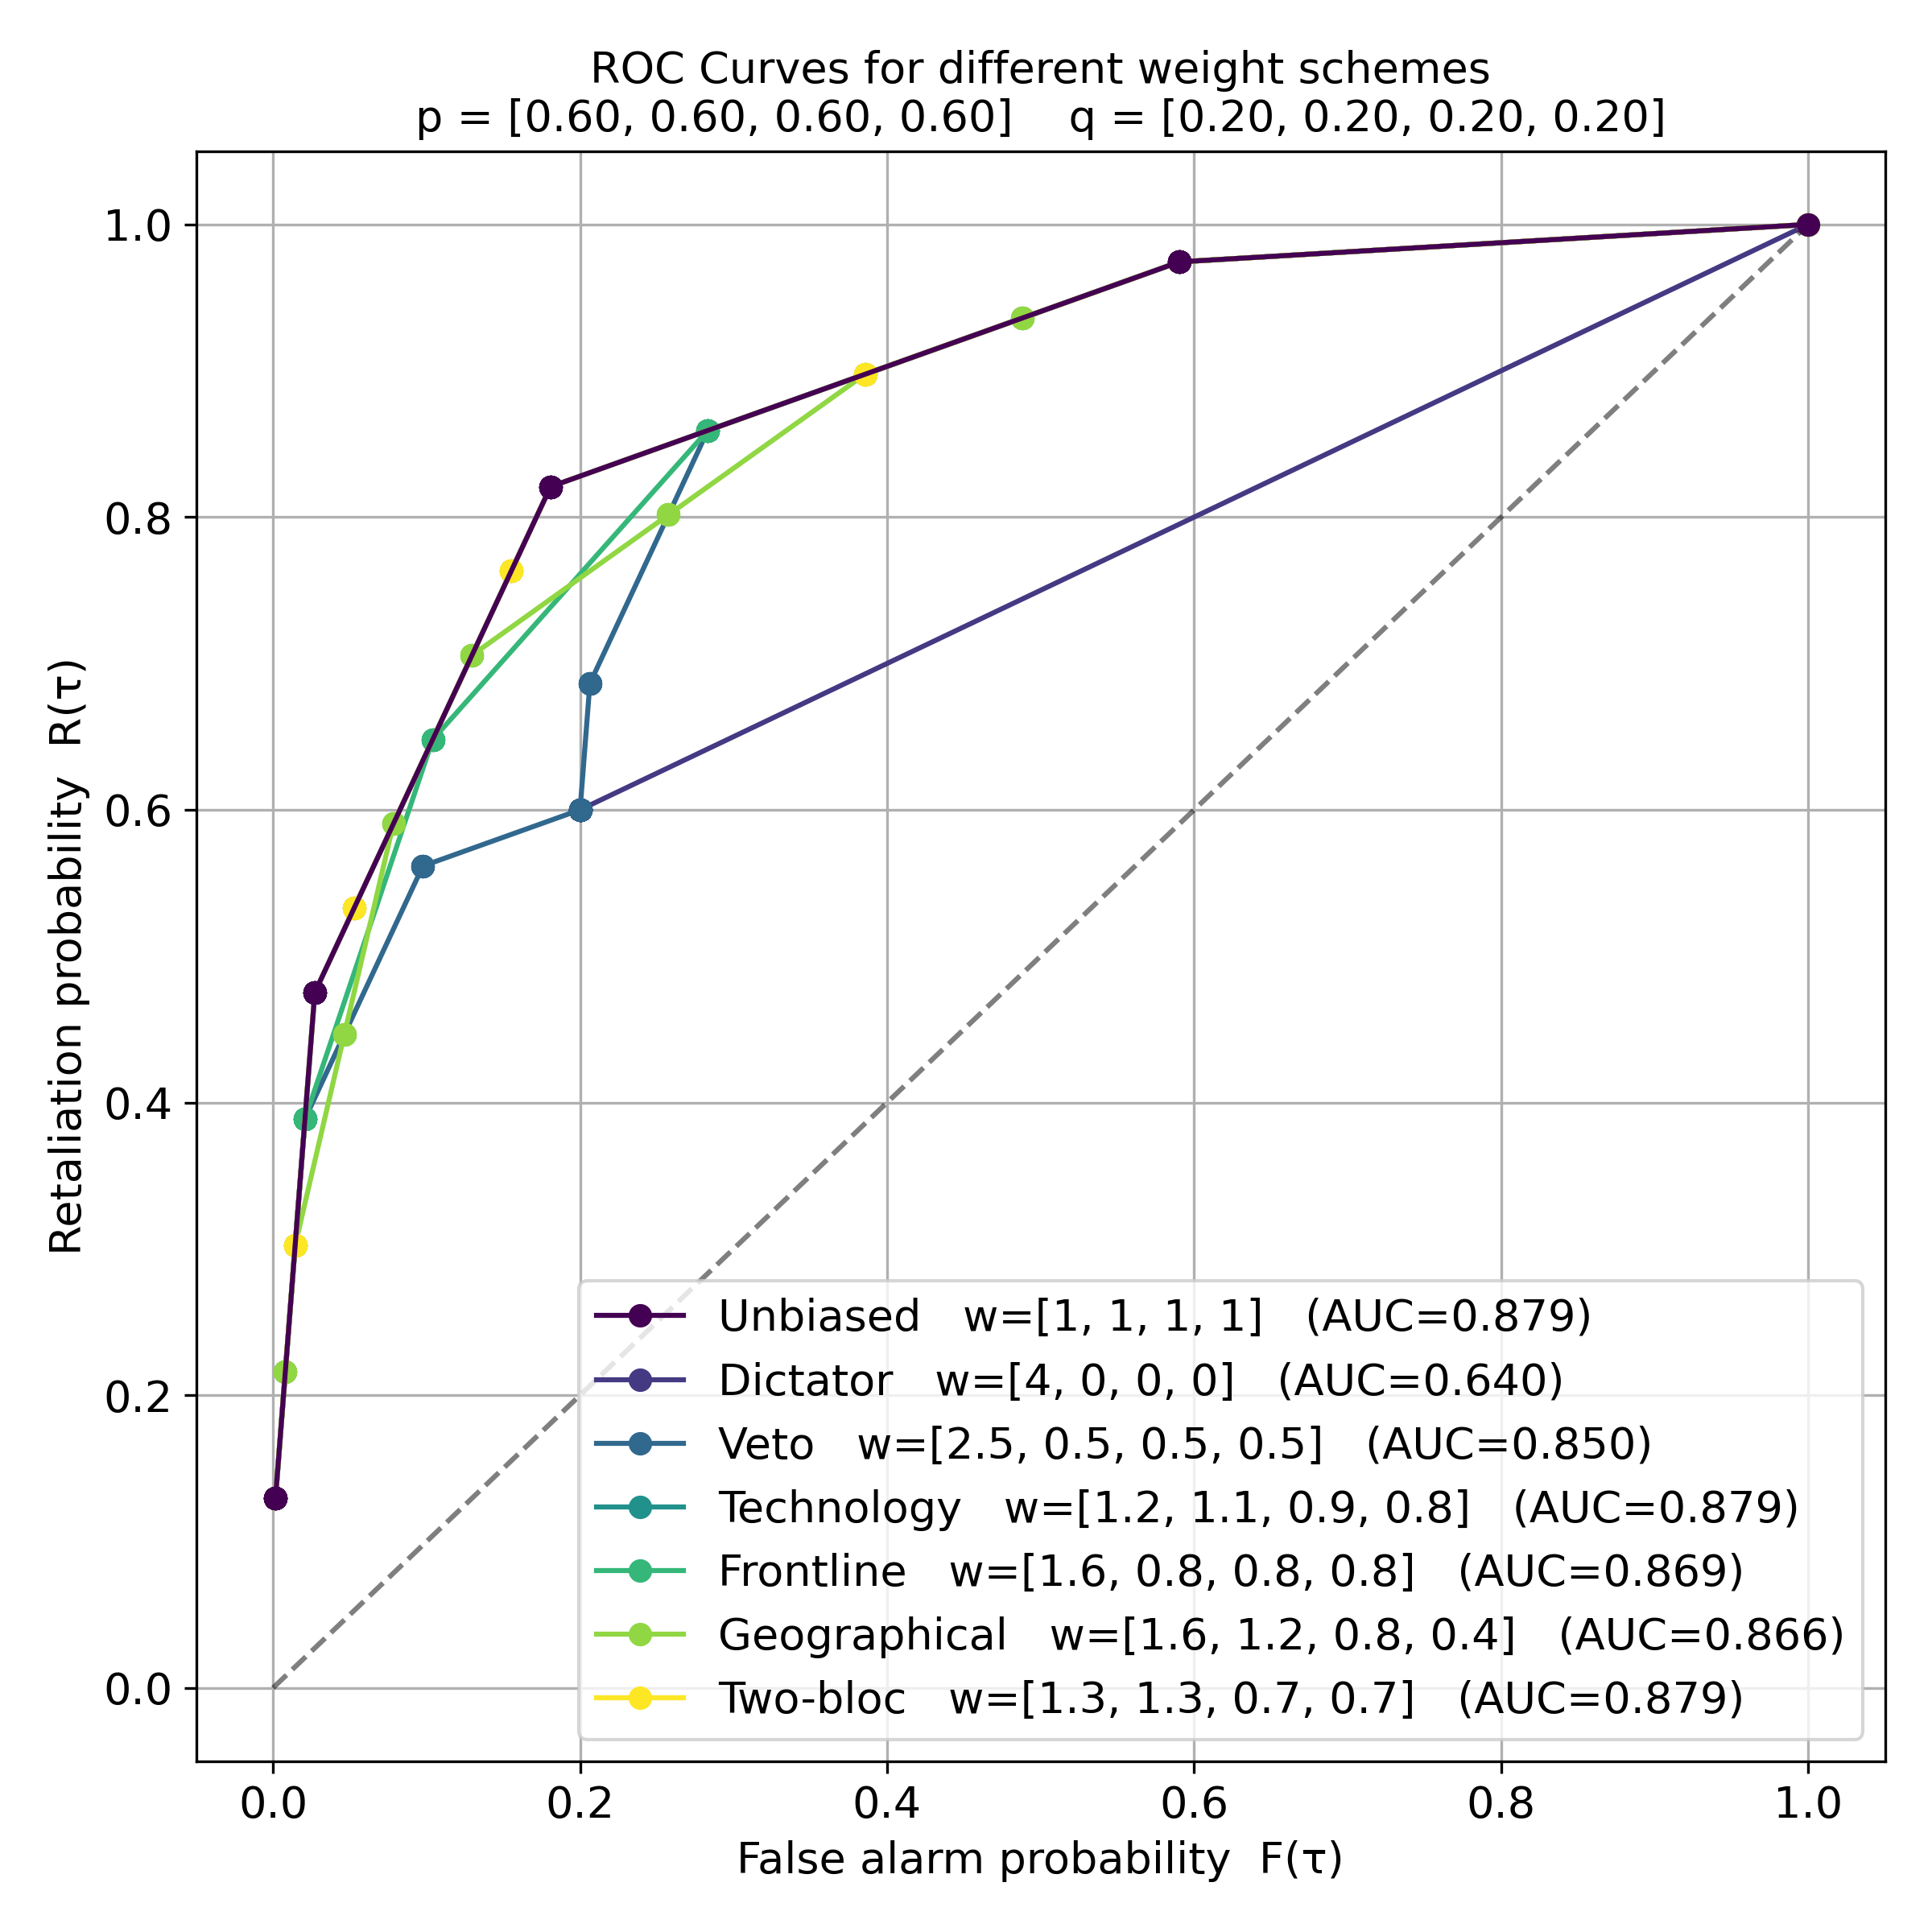
\includegraphics[width=\columnwidth]{images/ROC_LowSymmetric.png.png}
    \label{fig:low-low}
\end{figure}

To differentiate a bit more, we consider the following increasin and probability-vectors, $p = [0.85, 0.70, 0.55, 0.40]$ and $q = [0.05, 0.10, 0.20, 0.30]$, as well as the misaligned vectors $p = [0.55, 0.65, 0.75, 0.85]$ and $q = [0.35, 0.25, 0.15, 0.05]$. 

\begin{figure}[h!]
    \centering
    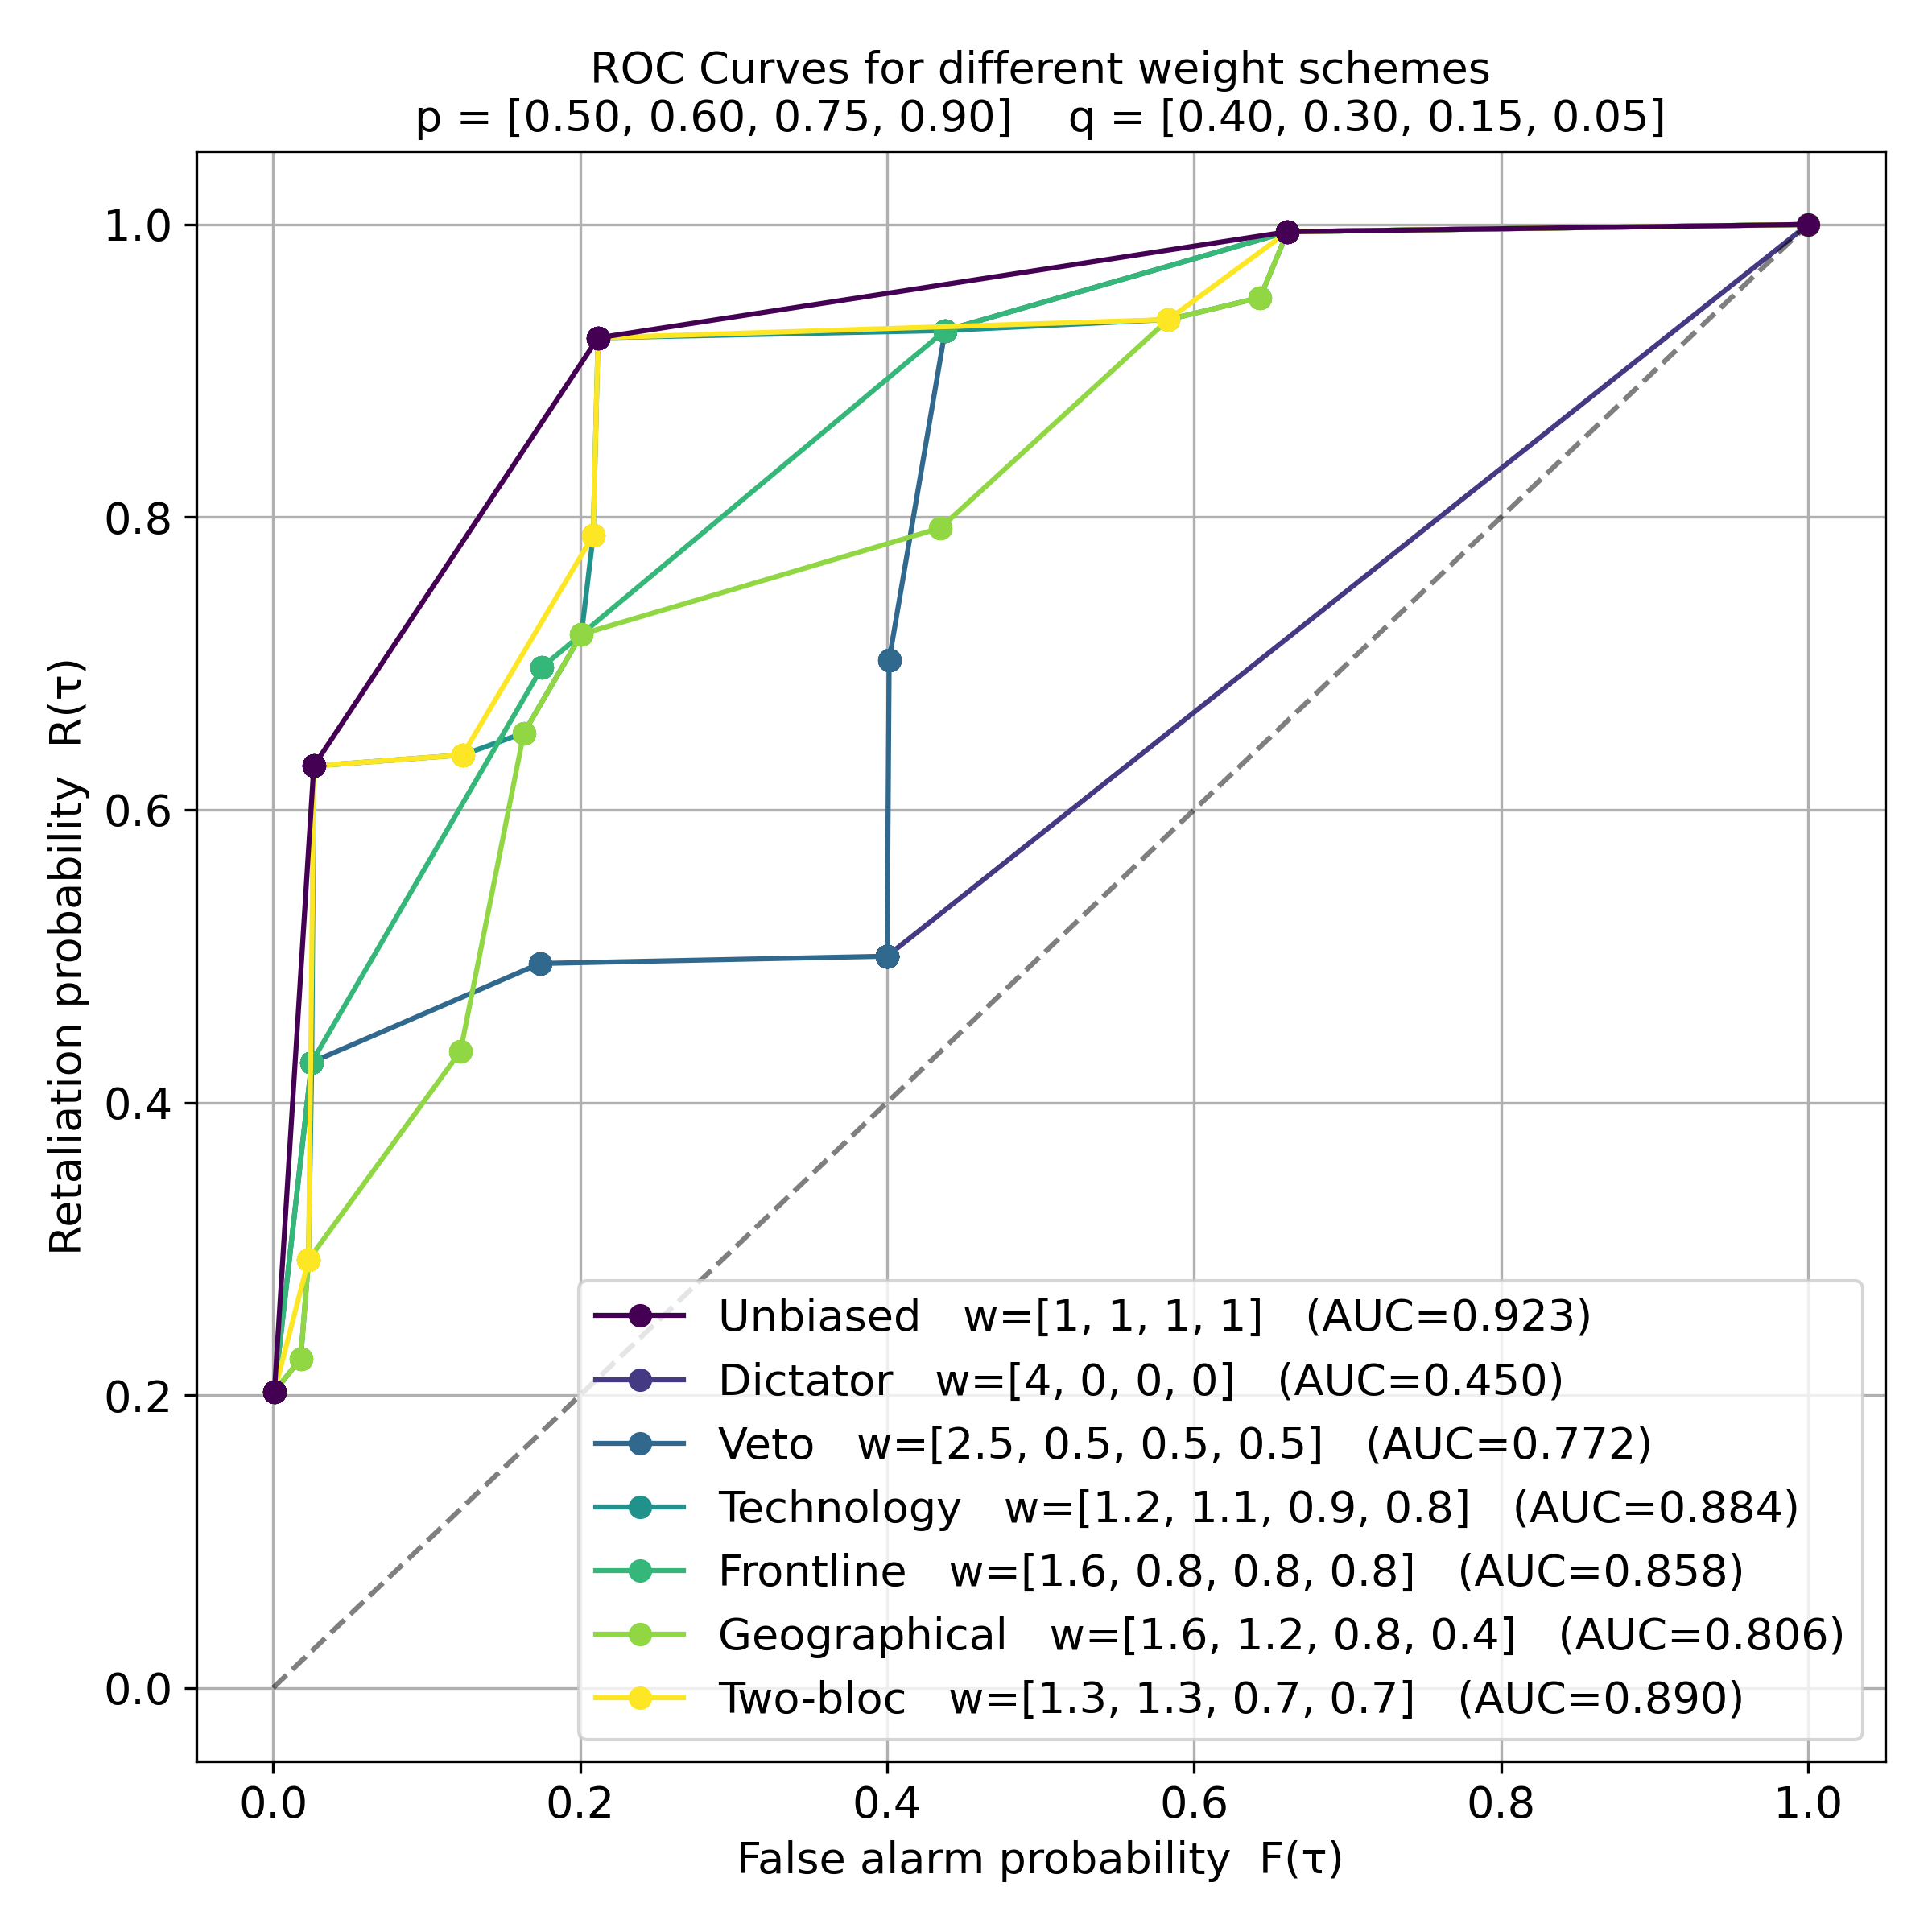
\includegraphics[width=\columnwidth]{images/ROC_IncreasingStrong.png.png}
    \label{fig:strong-increasing}
\end{figure}

\begin{figure}[h!]
    \centering
    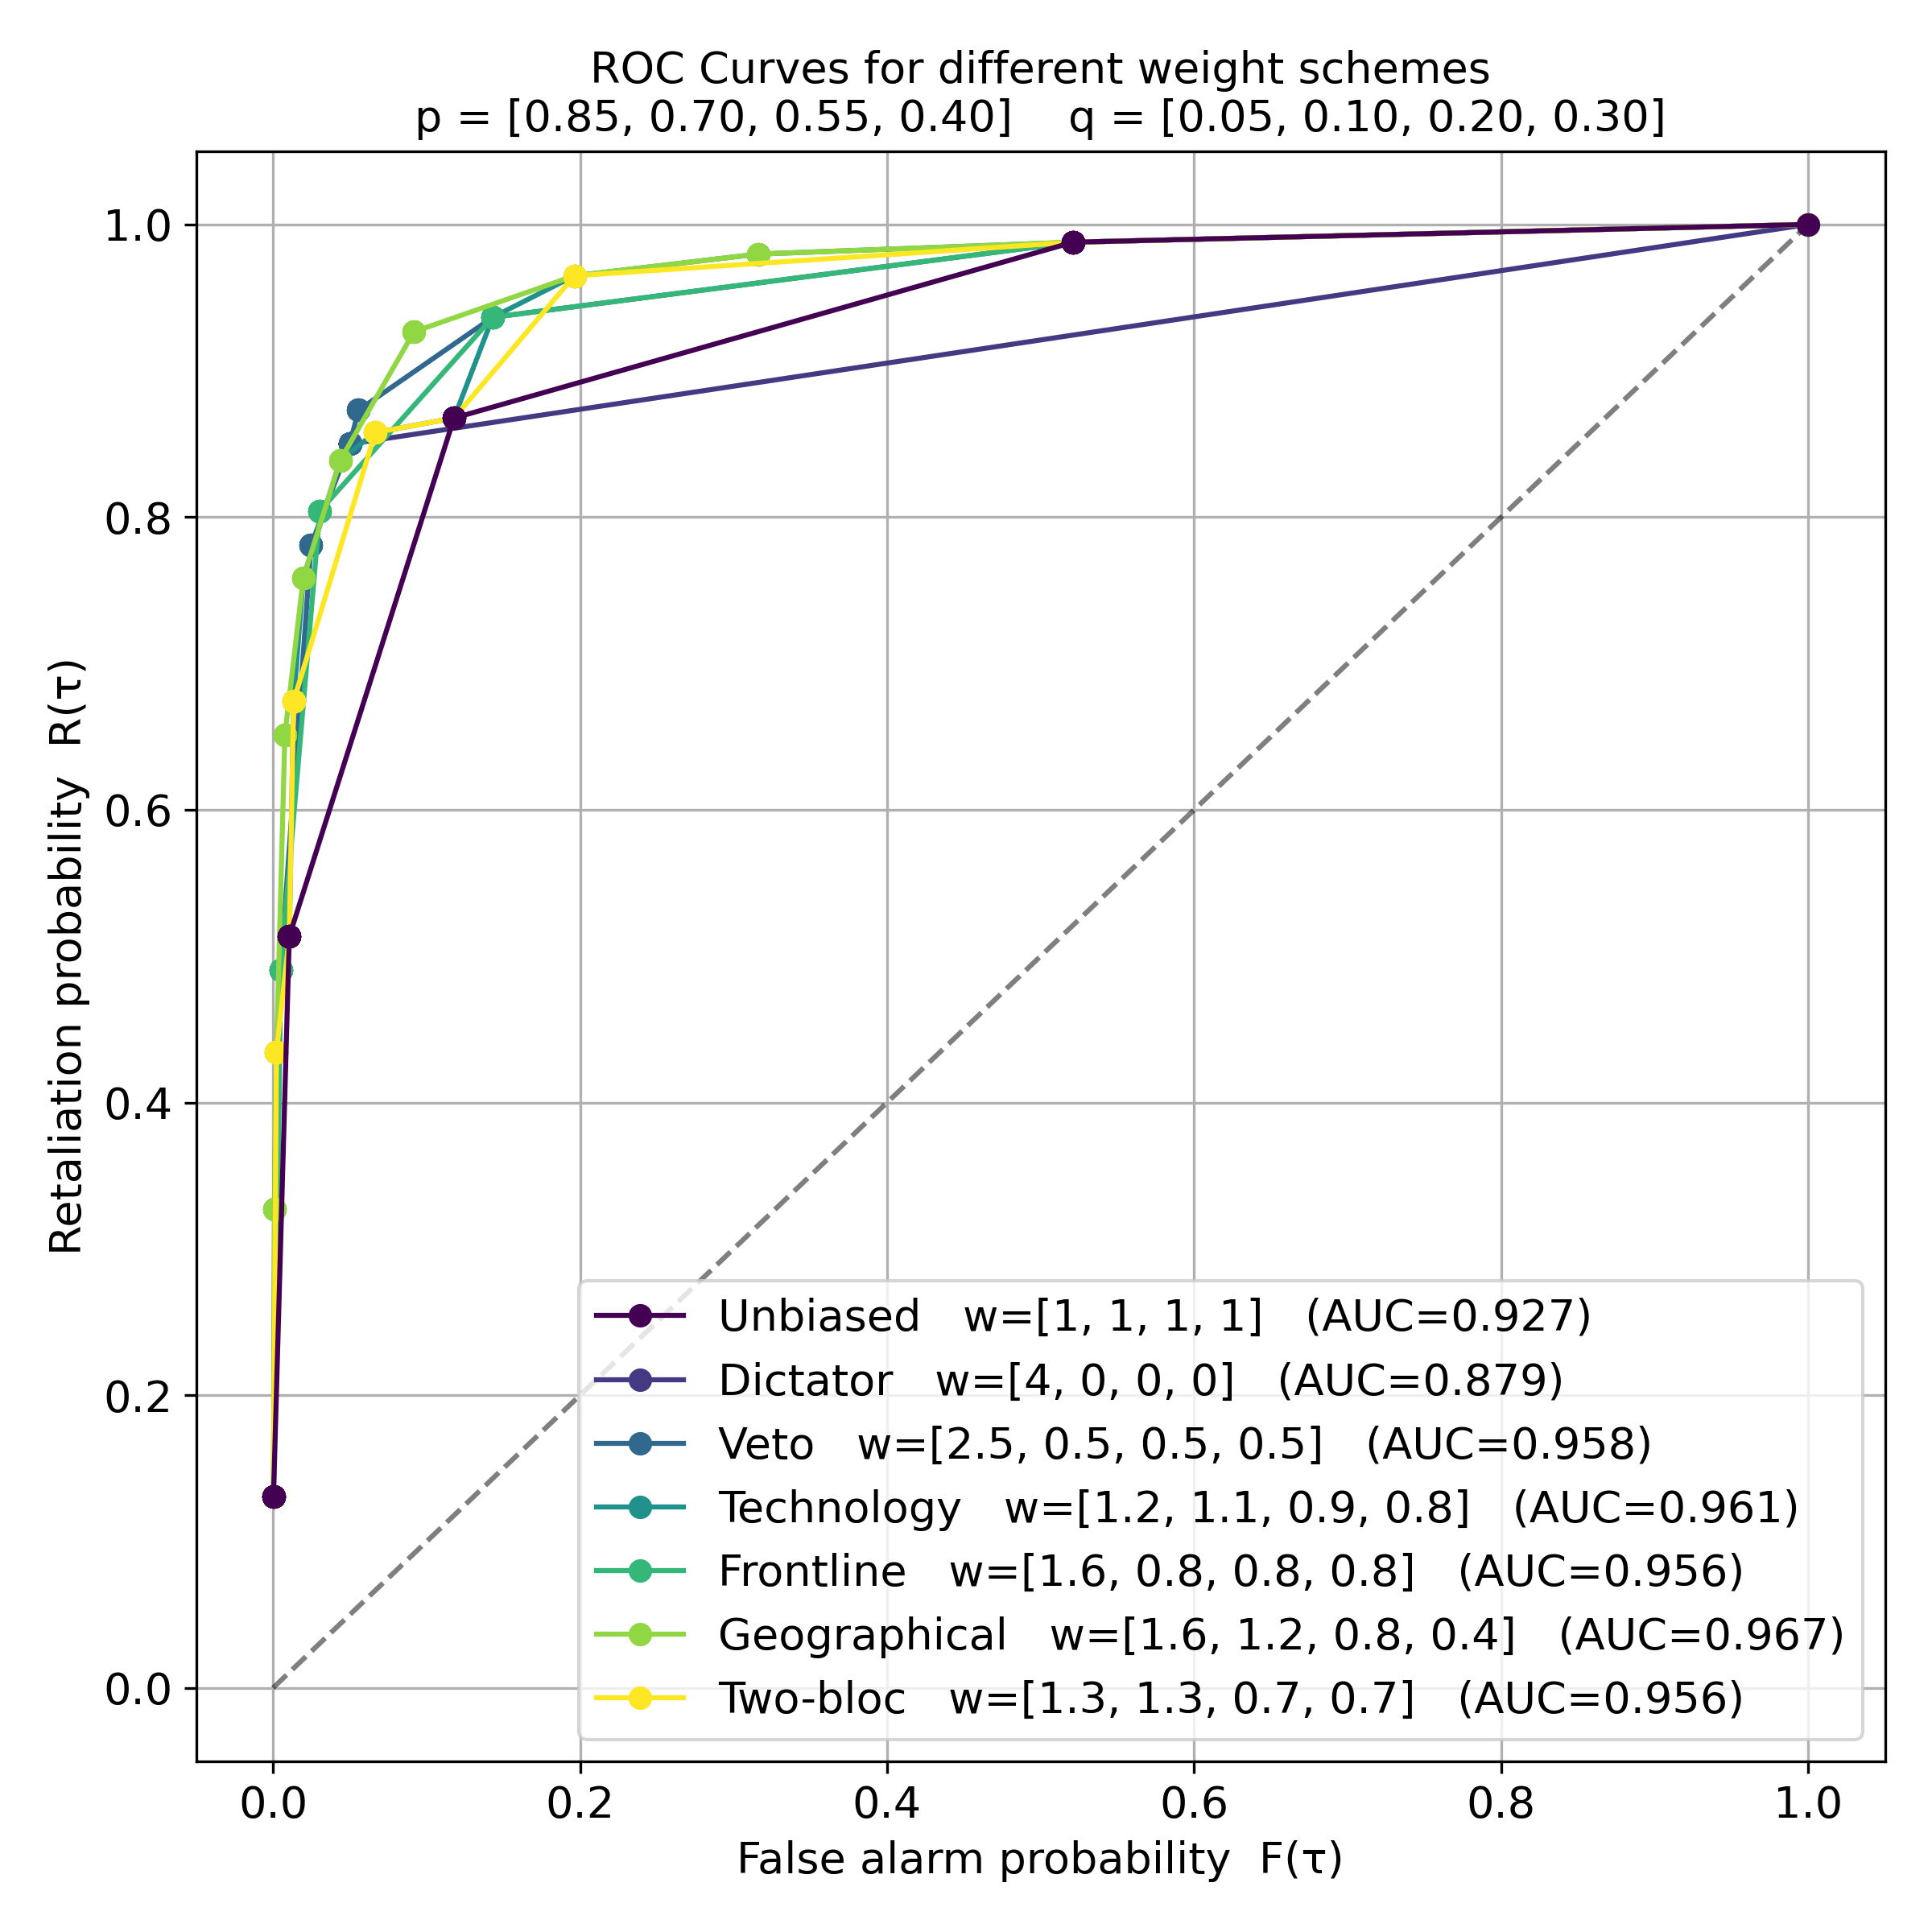
\includegraphics[width=\columnwidth]{images/ROC_StrongDecreasing.png.png}
    \label{fig:strong-decreasing}
\end{figure}

As one can see, some of the weight schemes are performing consistently better than others. To veryfy this we evaluate the weight schemes on a large variety of probability vectors, listed below, and study the statistics of their AUCs. We use 
\begin{table}[h!]
\label{table:p-q-vectors}
\centering
\begin{tabular}{c c}
\hline
\textbf{$p$ vector} & \textbf{$q$ vector} \\
\hline
$(0.85, 0.85, 0.85, 0.85)$ & $(0.05, 0.05, 0.05, 0.05)$ \\
$(0.75, 0.75, 0.75, 0.75)$ & $(0.10, 0.10, 0.10, 0.10)$ \\
$(0.60, 0.60, 0.60, 0.60)$ & $(0.20, 0.20, 0.20, 0.20)$ \\
$(0.90, 0.80, 0.70, 0.60)$ & $(0.05, 0.10, 0.15, 0.20)$ \\
$(0.85, 0.70, 0.55, 0.40)$ & $(0.05, 0.10, 0.20, 0.30)$ \\
$(0.60, 0.65, 0.70, 0.75)$ & $(0.25, 0.20, 0.15, 0.10)$ \\
$(0.55, 0.65, 0.75, 0.85)$ & $(0.35, 0.25, 0.15, 0.05)$ \\
$(0.50, 0.60, 0.75, 0.90)$ & $(0.40, 0.30, 0.15, 0.05)$ \\
$(0.55, 0.55, 0.55, 0.55)$ & $(0.45, 0.45, 0.45, 0.45)$ \\
$(0.85, 0.55, 0.80, 0.50)$ & $(0.05, 0.25, 0.10, 0.30)$ \\
$(0.90, 0.88, 0.60, 0.50)$ & $(0.05, 0.06, 0.25, 0.30)$ \\
$(0.72, 0.58, 0.81, 0.63)$ & $(0.11, 0.22, 0.07, 0.19)$ \\
$(0.78, 0.82, 0.79, 0.40)$ & $(0.12, 0.10, 0.11, 0.35)$ \\
$(0.88, 0.55, 0.70, 0.83)$ & $(0.06, 0.28, 0.18, 0.10)$ \\
\hline
\end{tabular}
\caption{Varied range of vectors used in the analysis.}
\end{table}

Computing AUC values for all of these, we obtain the following statistics for each weight scheme. 

\begin{table}[h!]
\centering
\begin{tabular}{lccc}
\hline
\textbf{Weight scheme} & \textbf{Mean} & \textbf{Min} & \textbf{Max} \\
\hline
Unbiased     & 0.932 & 0.606 & 0.998 \\
Dictator     & 0.719 & 0.426 & 0.903 \\
Veto         & 0.902 & 0.594 & 0.991 \\
Technology   & 0.931 & 0.606 & 0.998 \\
Frontline    & 0.922 & 0.602 & 0.996 \\
Geographical & 0.914 & 0.600 & 0.988 \\
Two-bloc     & 0.929 & 0.606 & 0.998 \\
\hline
\end{tabular}
\caption{Mean, minimum and maximum AUC values for each weight scheme, computed from the probability-vectors listed in \cref{table:p-q-vectors}.}
\end{table}

The best performer is the unbiased weight scheme, followed closely by the technology scheme and the two-bloc scheme. The dictator scheme performs considerably worse than the others. The following show the top two performers, and the worst performer, mapped against all the probability vectors in \cref{table:p-q-vectors}. 

\begin{figure}[h!]
    \centering
    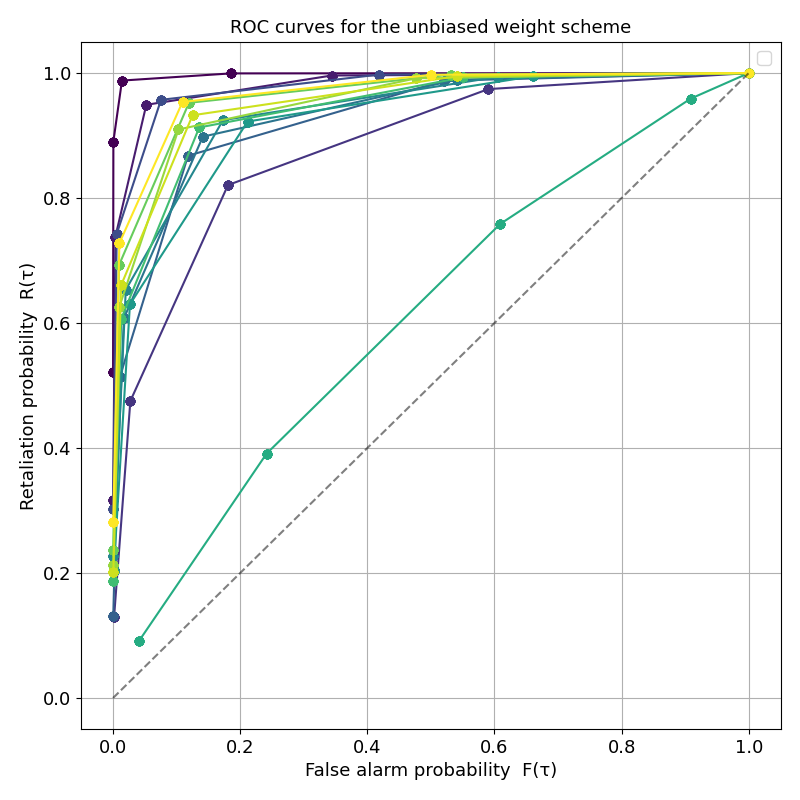
\includegraphics[width=\columnwidth]{images/unbiased_no-label.png}
    \label{fig:unbiased}
\end{figure}

\begin{figure}[h!]
    \centering
    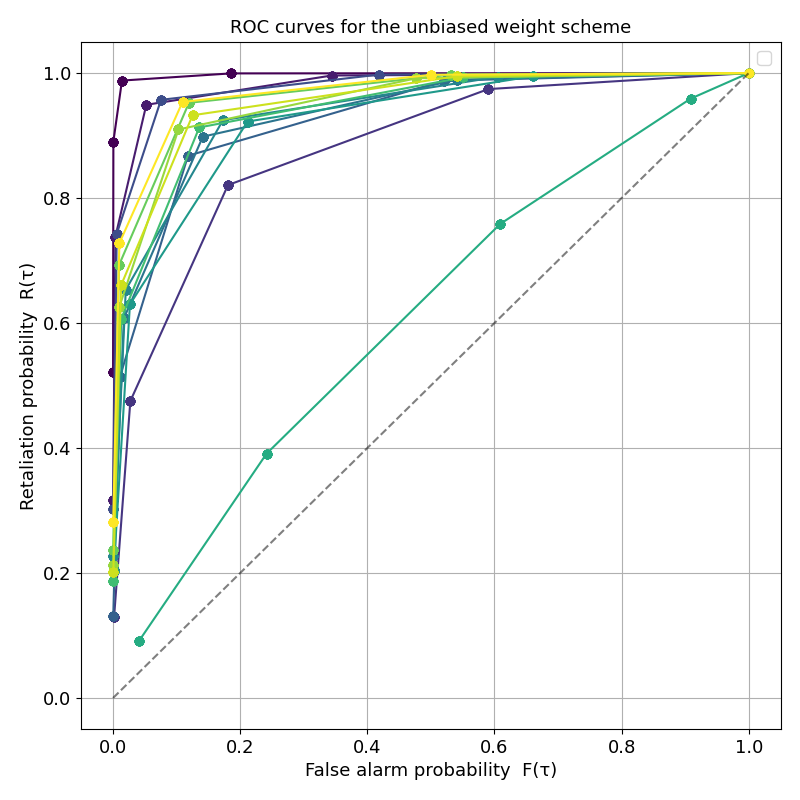
\includegraphics[width=\columnwidth]{images/unbiased_no-label.png}
    \label{fig:technology}
\end{figure}

\begin{figure}[h!]
    \centering
    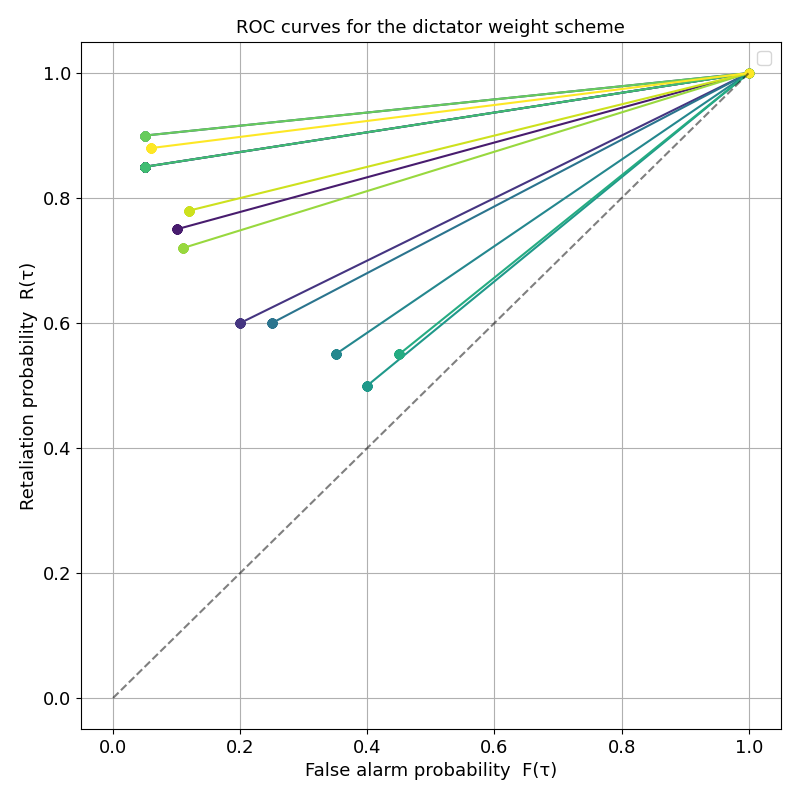
\includegraphics[width=\columnwidth]{images/dictator_no-label.png}
    \label{fig:dictator}
\end{figure}






\subsection{Large coalitions}